\section{Evaluation}
\label{sec-evaluation}

\XXXnote{GWA: TODO: Integrate.}


\subsection{Detector Experiment}

\begin{figure}
\centering
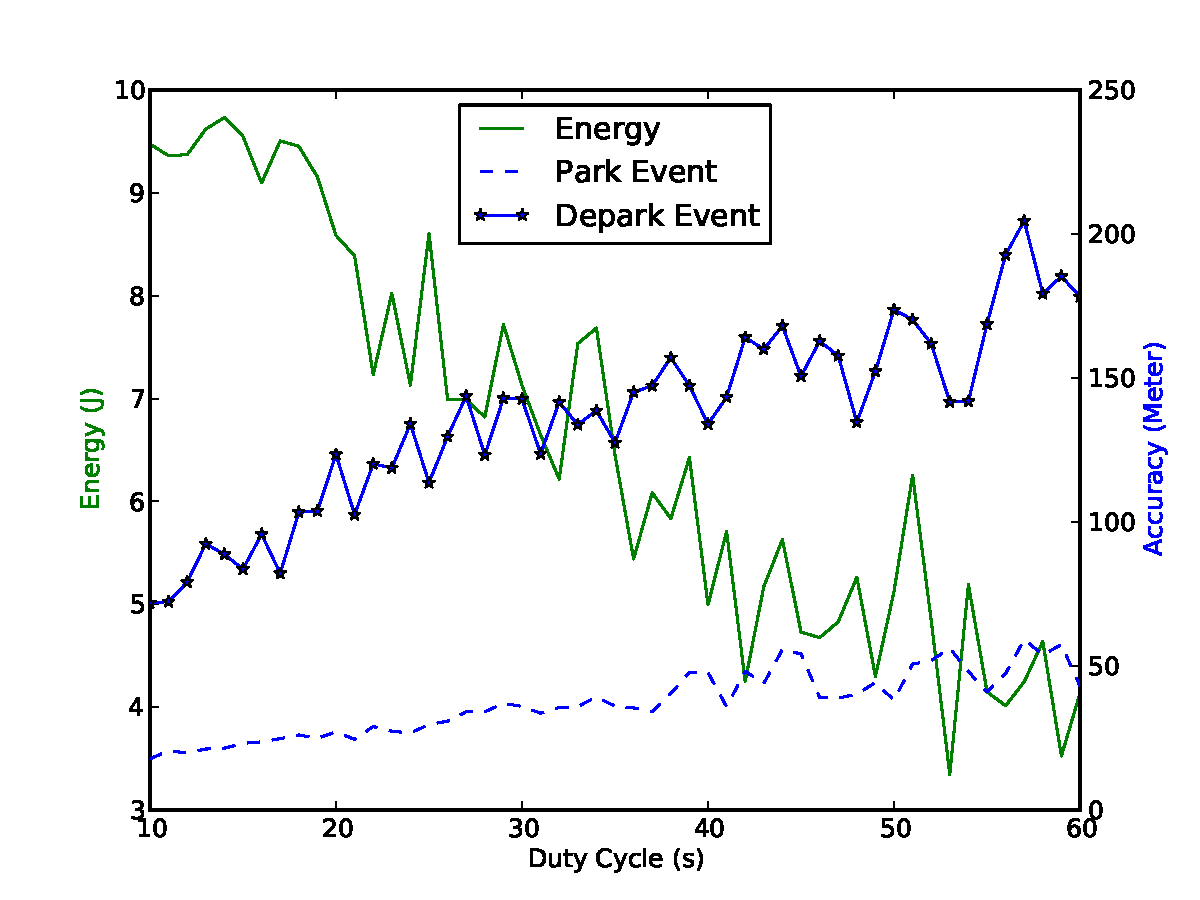
\includegraphics[width=\columnwidth]{./figures/Energy_accuracy.pdf}

\caption{\textbf{Power usage vs. detector accuracy.} \XXXnote{GWA: TODO.}}

\label{fig-energy}
\end{figure}

\newcolumntype{b}{>{\hsize=1.4\hsize}X}
\newcolumntype{s}{>{\hsize=.6\hsize}X}
\begin{table}[t]
{\small
\begin{threeparttable}
\begin{tabularx}{\columnwidth}{b s b s}
  {{\textbf{Carry Location}}} & {{\textbf{Count}}} &
  {{\textbf{Car Location}}} &
  {{\textbf{Count}}} \\
 \hline
In hand & 18 & Cup holder & 16 \\
Side bag & 10 & Car seat  & 9 \\
Back pack & 10 & Side bag & 10 \\
In hand talking & 7 & Back pack & 9 \\
Front pocket & 14 & Front pocket & 14 \\
Jacket pocket & 14 & Jacket pocket & 14 \\
Back pocket & 7 & Back pocket & 14 \\
\end{tabularx}
\end{threeparttable}
\caption{\textbf{Carry and car location for detector experiment.}
Eight participants generated 80 runs, carrying and placing the
phone in their car in many ways.}
\label{table-experiment}
}
\vspace*{-0.1in}
\end{table}


To furnish further ground truth, we conducted a structured experiment on March
17th. Eight volunteers participated, including seven men and one woman, seven 
of whom were right-handed and one of whom was left-handed.
Each was asked to conduct the same experiment:  carrying a mobile phone, walk
out to his car, drive around briefly, park and walk back inside.  Each
participant was further instructed to repeat this experiment ten times,
following set directions as to where to hold or carry the phone while walking
and driving.  Participants spent approximately three to five minutes per run
for a total of slightly under an hour total for the entire experiment.

The experiment permitted us to obtain sensing data from a cross section of
people posessed of varying body morphologies and different habits of driving
cars and handling mobile devices.

\subsection{Simulation Results}

\begin{figure*}
\centering
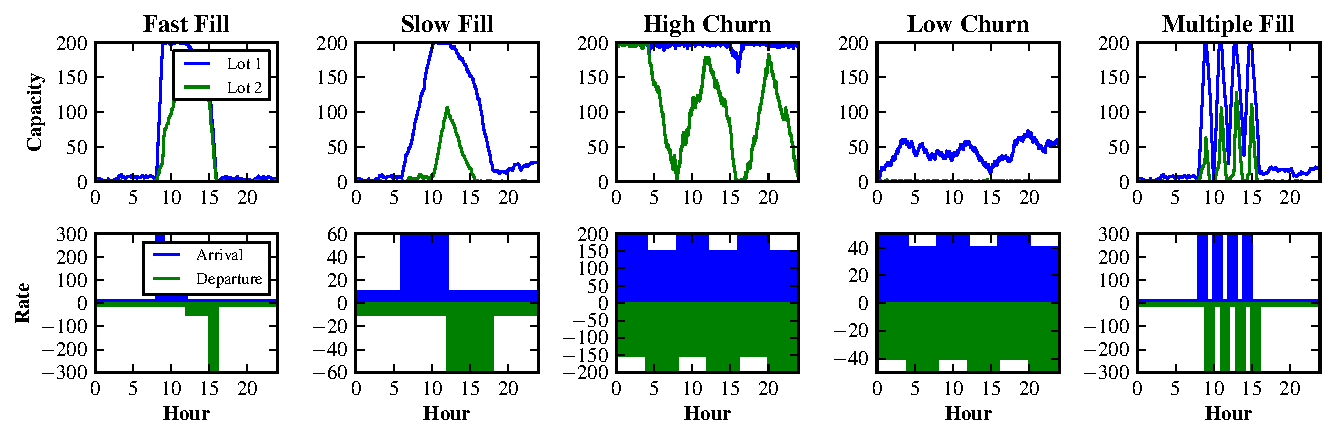
\includegraphics[width=\textwidth]{./simulator/figures/lots.pdf}

\caption{\textbf{Description of each type of lot simulated.} \XXXnote{GWA:
TODO.}}

\label{fig-lotsdescription}
\end{figure*}

\begin{figure*}
\centering
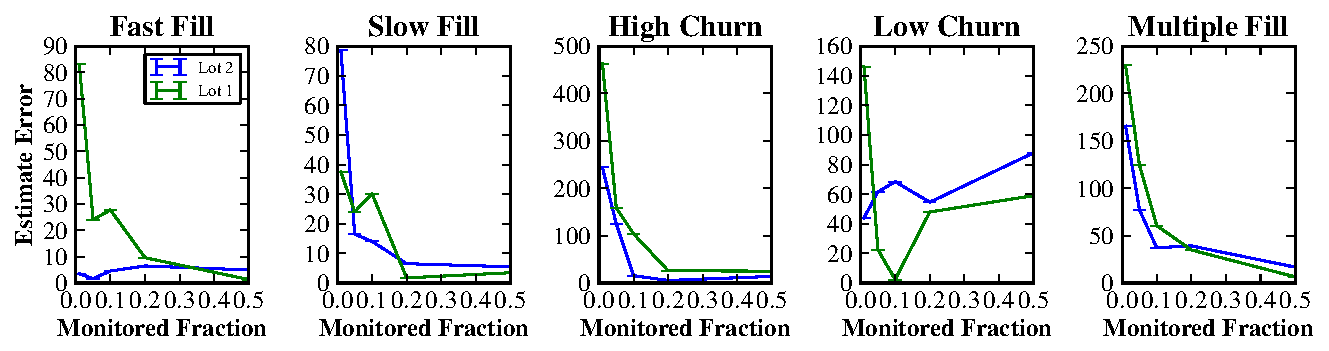
\includegraphics[width=\textwidth]{./simulator/figures/capacity_experiment.pdf}

\caption{\textbf{Errors in capacity estimation.} \XXXnote{GWA: TODO.}}

\label{fig-capacityerrors}
\end{figure*}

\begin{figure}
\centering
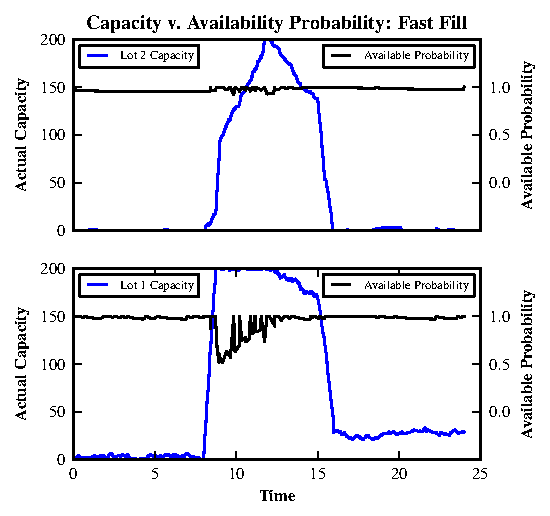
\includegraphics[width=3.0in]{./simulator/figures/tracking_fastfill.pdf}

\caption{\textbf{Availability probabilities tracking lot capacity.} \XXXnote{GWA: TODO.}}

\label{fig-trackingexample}
\end{figure}


\subsection{Deployment}

\begin{figure*}
\centering
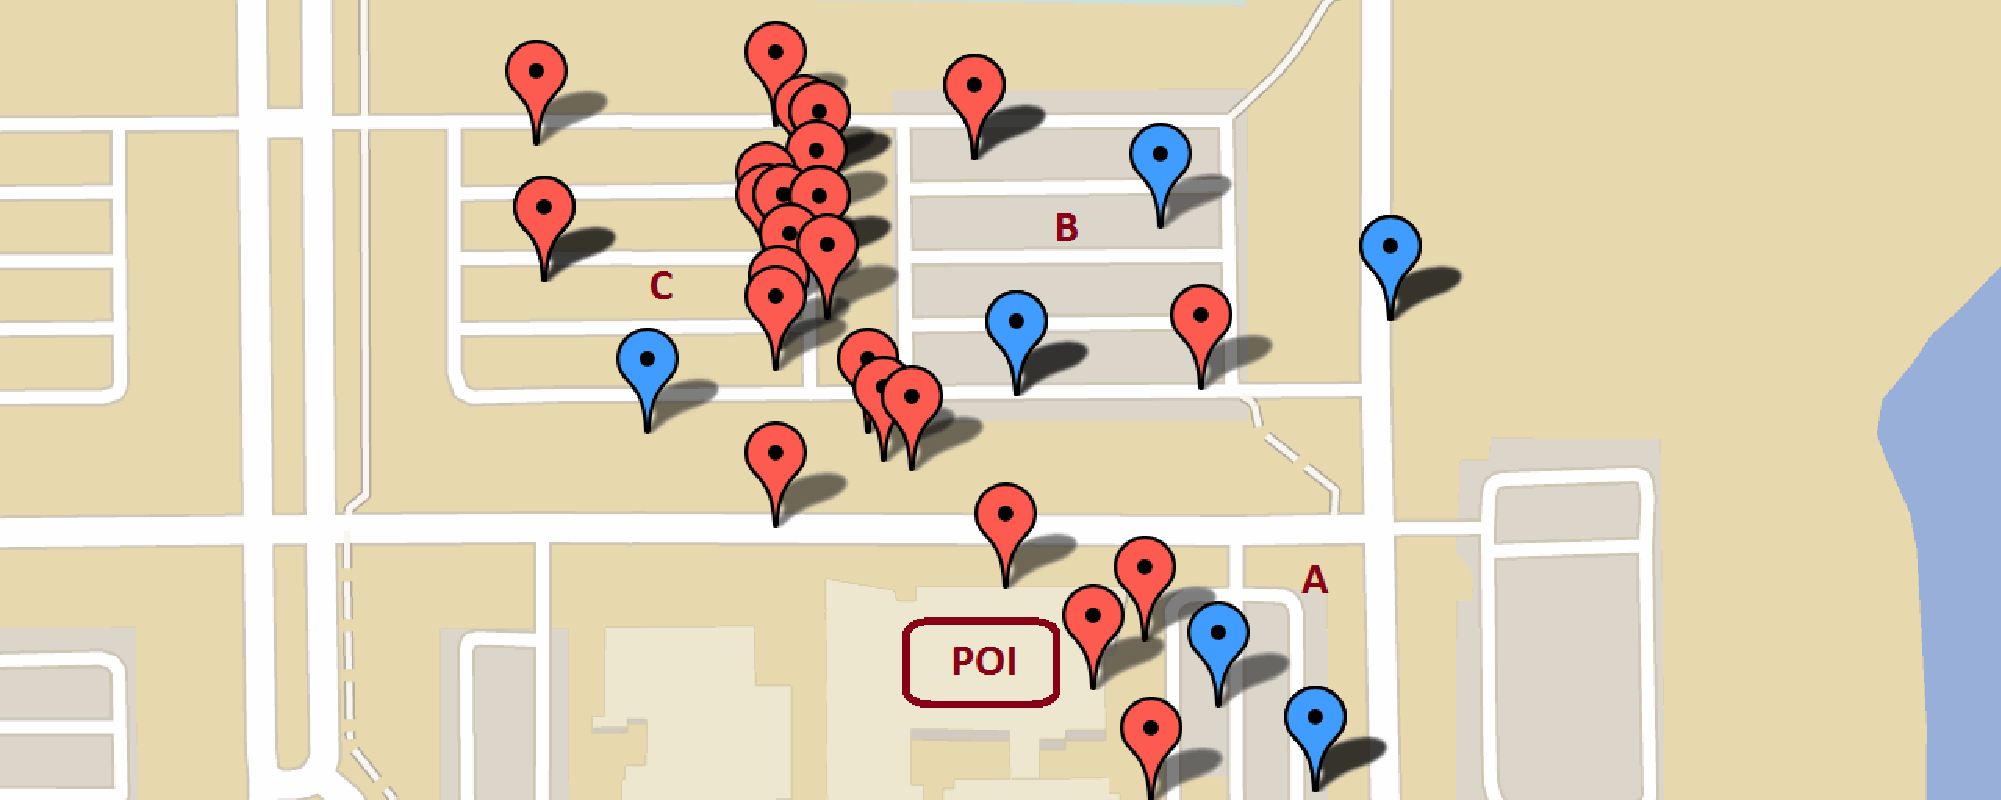
\includegraphics[width=\textwidth,height=2in]{./figures/detectedEventsOnMap.pdf}

\caption{\textbf{Map showing all events detected by PocketParker during our
deployment.} \XXXnote{GWA: TODO.}}

\label{fig-energy}
\end{figure*}

\begin{figure}
\centering
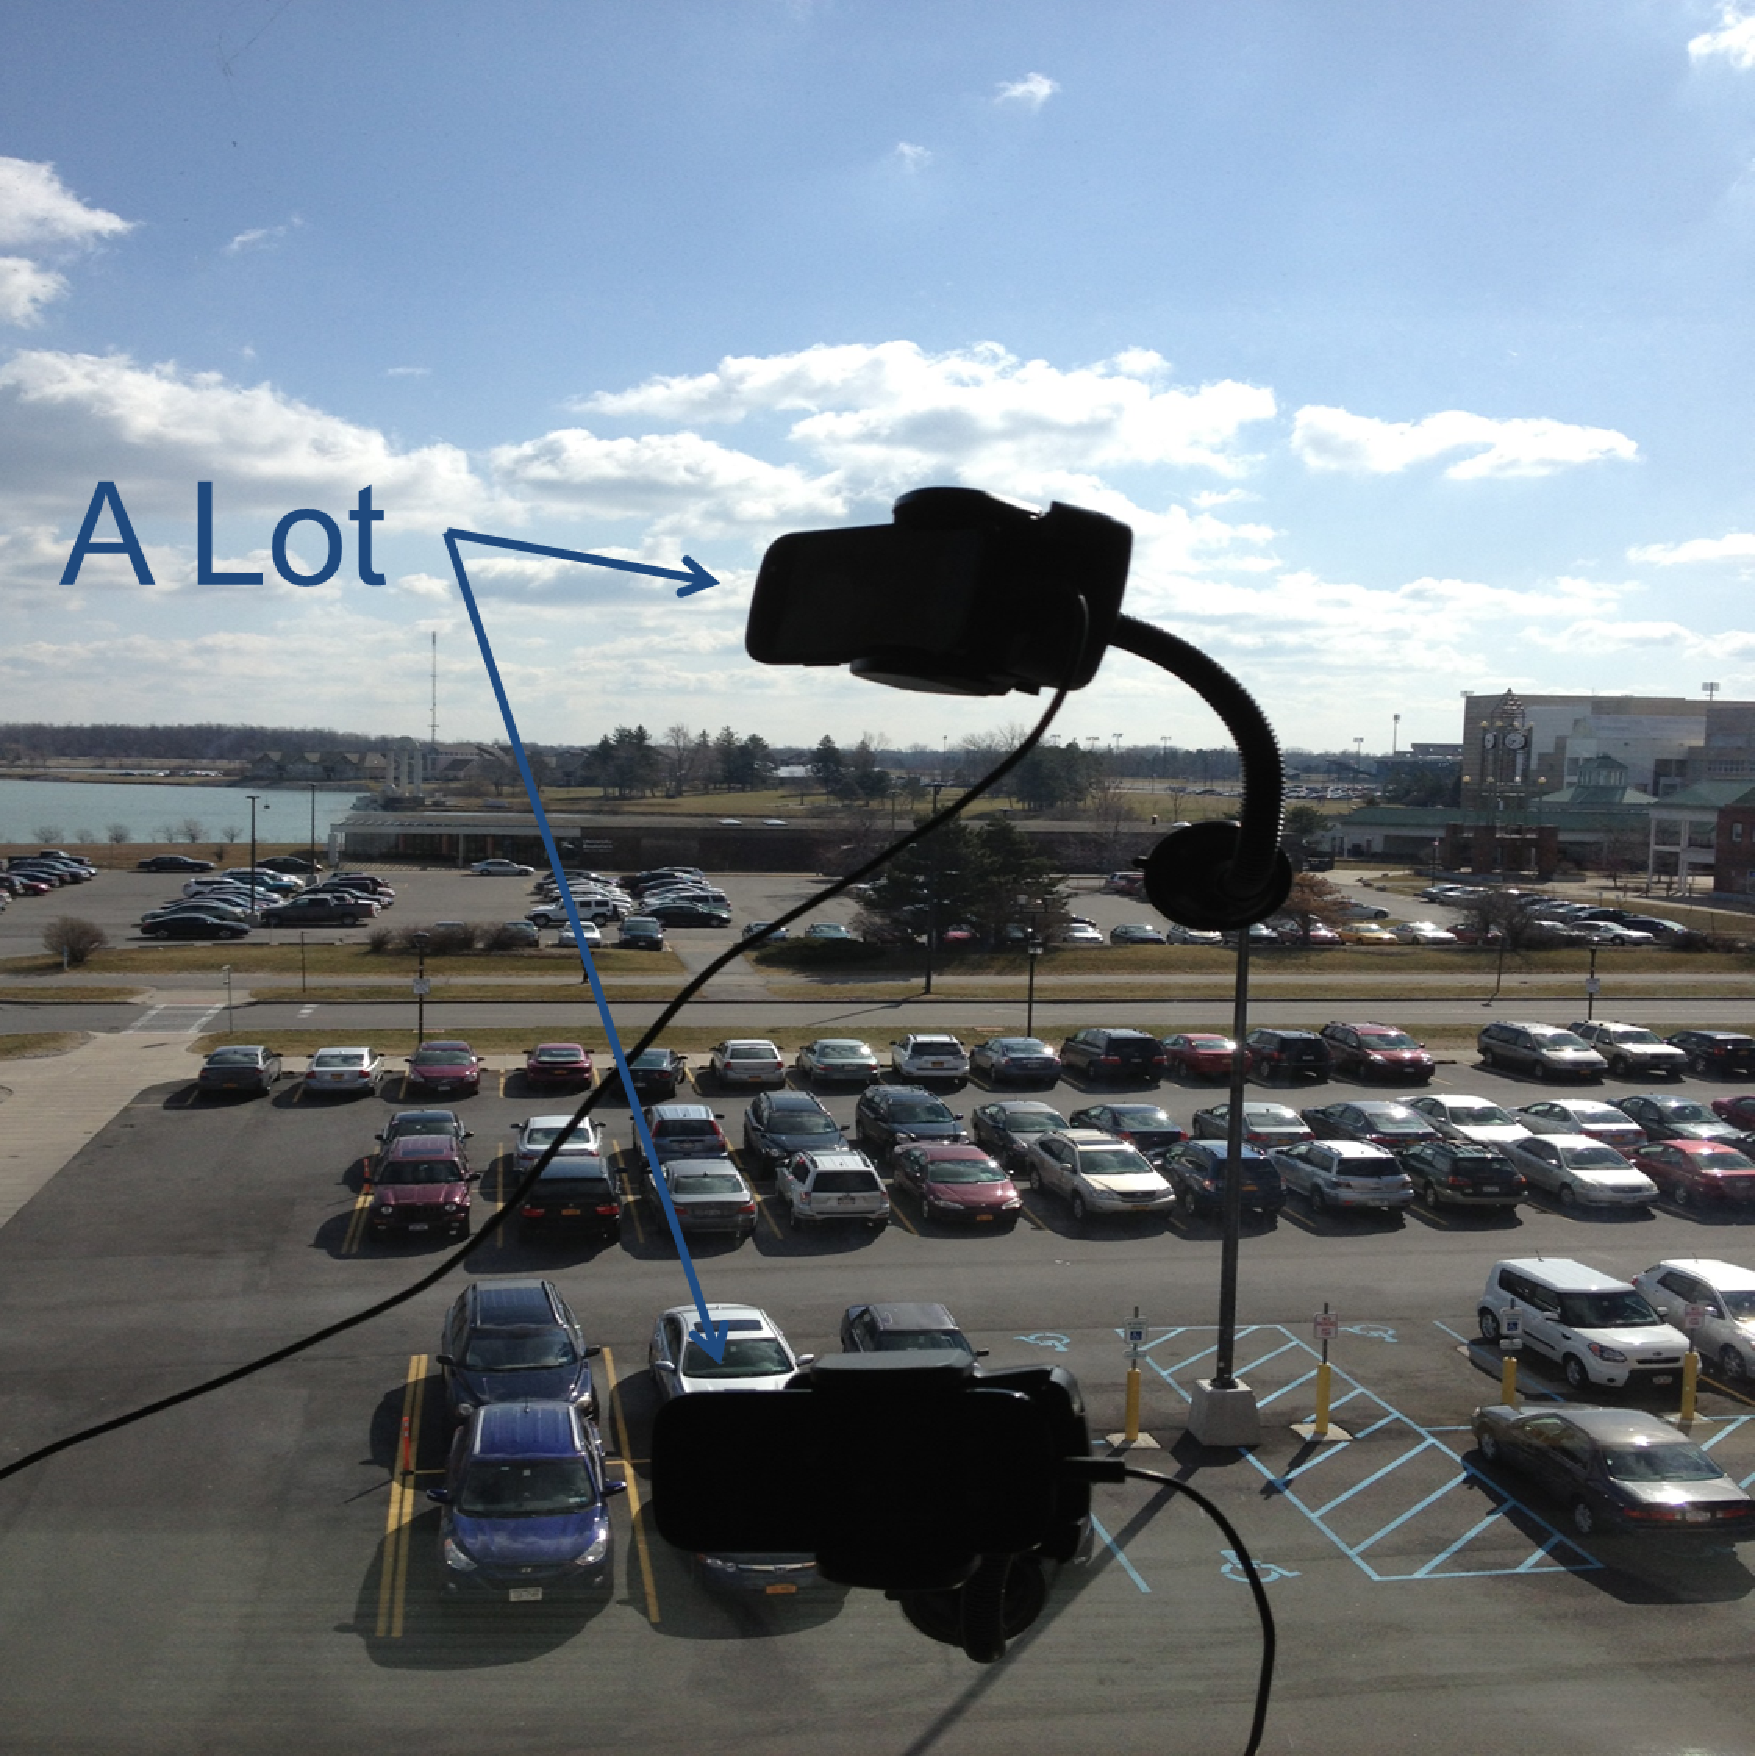
\includegraphics[width=\columnwidth]{./figures/Camera_setting.pdf}

\caption{\textbf{Monitoring cameras.} A view of one of the monitored parking
lots is shown.}

\label{fig-camera}
\end{figure}
